%!TEX root = ../Thesis.tex
\chapter{Linking brain-wide gene expression and neuroimaging data}
\label{appendixB}
\fancyhead[R]{\textit{Appendix B:~Linking brain-wide gene expression and neuroimaging data}}

\section{Details on AHBA}
\label{app:AppendixCh4_1}

\textbf{Details on AHBA}\\
The AHBA microarray gene expression data consists of \num{3702} samples from six  neurotypical adult brains. Several hundred samples (mean $\pm$ standard deviation: 617 $\pm$ 241) were collected from cortical, subcortical, brainstem and cerebellar regions in each brain and profiled for genome-wide gene expression using custom Agilent $8\times60$K cDNA chip which consists of a standard Whole Human Genome Microarray Kit, $4\times44$K (Design ID: 014850) and more than \num{18000} custom-generated probes created specifically for AHBA in order to increase the genetic coverage. Originally, \num{48171} of all \num{58692} probes were annotated to a gene, resulting in a set of \num{20787} unique genes with expression measures. In addition to gene expression data, the AHBA provides a binary indicator when the level of a given transcript exceeds background [as defined by the $t$-test -based criteria \citep{AHBAdoc}].
Each probe in the AHBA is associated with a numerical ID and a platform-specific label or name. If a probe is assigned to represent a unique gene it is also characterized with a range of gene-specific labels such as gene symbol and an entrez gene ID, a stable identifier for a gene generated by the Entrez Gene database at the National Center for Biotechnology Information (NCBI). If required, probe sequences can be accessed using the Allen Institute’s website application programming interface (see \ref{app:AppendixCh4_7}) while Agilent probe sequences can also be downloaded through the manufacturer's website (\url{https://earray.chem.agilent.com/earray/}). Probe sequences can also be found in the figshare repository \url{https://doi.org/10.6084/m9.figshare.6852911}. Note that the expression levels of a single gene can be measured using multiple probes that correspond to a different part of the gene sequence. In the AHBA, 93\% of all genes are annotated to more than one probe.

Probe-level data are available for each of \num{3702} tissue samples taken throughout the brain. Different brain regions were sampled across each of the six AHBA donors to maximize spatial coverage. Each tissue sample is associated with a numeric structure ID, name, and structure label (`cortex', `cerebellum', or `brainstem') in addition to the MRI voxel coordinates in native image space and MNI coordinates in standard space that can be used for matching samples to the stereotaxic space. The AHBA also provides RNA-seq data for a subset of tissue samples in two donor brains ($n=120$ each). It consists of expression values for more than \num{22000} genes presented in fragment count (number of reads matching a given gene) and TMP (Transcripts Per Kilobase Million -- normalized read count with regards to read and transcript length) formats. RNA-seq method quantifies the transcription by directly sequencing each molecule in high-throughput manner, therefore providing a more precise measurement of levels of transcripts without the prior knowledge of the DNA sequence of interest \citep{Wang2009}.

Magnetic resonance images--T1-weighted, T2-weighted, T2-weighted gradient echo and FLAIR--were collected prior to dissection of each brain for anatomic visualization. Diffusion tensor images were collected for two brains (H0351\_2001 and H0351\_2002). Detailed information about image acquisition sequences is presented in a technical white paper \citep{AHBAdoc}.


\section{Intensity-based filtering and RNA-seq}
\label{app:AppendixCh4_2}

\textbf{Enrichment analysis} \\
\noindent Software: version 3.1.2 version of ErmineJ software \citep{Gillis2010};\\
Biological process GO annotations: obtained from GEMMA \citep{Zoubarev2012} as \\
\texttt{Generic\_human\_ncbiIds\_noParents.an.txt} downloaded on May 16, 2018. \\
Gene Ontology terms and definitions: obtained from \url{archive.geneontology.org/latest-termdb/go_daily-termdb.rdf-xml.gz} on May 16 2018.\\
The analyses were performed only on the biological process annotations. \\

\textbf{Intensity-based filtering}\\
To test if intensity-based filtering (where probes are filtered based on the binary indication of expression levels exceeding the background) targets any specific functional gene groups, we performed the gene score resampling (GSR) analysis. Avoiding the potential bias of overestimating the influence of genes that are represented with multiple probes scores for the GRS analysis were determined at gene (rather than probe) level by: (i) calculating the proportion of samples with expression values exceeding the background using the binary indicator provided by AHBA for each probe; (ii) if more than one probe was available for a gene, the probe with the highest proportion of samples exceeding the background was selected to represent that gene. As a result, each of the \num{20232} genes was assigned a score indicating the proportion of samples with expression levels exceeding the background. The analysis was performed focusing on genes with low scores in order to determine what functional gene groups are affected by intensity-based filtering. The mean score in a GO group was selected to summarize it, using full resampling with $10^{6}$ iterations. FDR-corrected $p$-values (across around \num{7000} GO categories) were used to summarize the effect. The significant GO categories (at $p_\mathrm{corr}<0.05$) include non brain-specific processes such as sensory perception, chemotaxis, cell killing, and immune response among others (a list of TOP 100 GO categories is presented in supplementary file enrichmentExpression.csv). \\

\textbf{RNA-seq – microarray non-overlap}\\
The usage of RNA-seq expression measures for probe selection in microarray data is limited to genes that are present in both datasets. Given that $\sim13\%$ ($n=$\num{2623}) out of the  \num{20232} genes in the microarray data are not present in the RNA-seq dataset, we aimed to characterize the types of genes that do not have corresponding RNA-seq measures, and test if any brain-specific functional groups of genes are over-represented in this set as these genes would be excluded from the further analysis. If this is the case, then probe selection based on the correlation to RNA-seq data would not be an optimal solution due to the loss of relevant information. Overrepresentation analysis (ORA) was performed for each biological process GO category with 5 to 100 genes available taking the mean score in a GO group to summarize it. FDR-corrected $p$-values (across around \num{7000} GO categories) were used to summarize the effect. The significant GO categories (at $p_\mathrm{corr}<0.05$) include general processes such as septin assembly and organization as well as the negative regulation of RNA splicing among others (presented in supplementary file enrichmentExpression.csv) and are not related to brain-specific biological processes. \\

\textbf{Microarray and RNA-seq correlation}\\
In order for RNA-seq gene expression measures to provide a valid reference when selecting a probe, microarray and RNA-seq measures should be at least weakly correlated. Given that for a number of genes the maximum correlation between microarray and RNA-seq expression measures is very low, the probe selection based on such low correlations will be invalid. Therefore, we first exclude probes exhibiting a low correlation (taking a selected threshold, $\rho < 0.2$) to RNA-seq data resulting in the exclusion of \num{6725} genes. To evaluate the functional groups of genes that were removed, we performed an overrepresentation analysis (ORA). Avoiding the potential bias of overestimating the influence of genes that are represented with multiple probes, scores for the ORA analysis were determined at gene (rather than probe) level by: (i) calculating correlation between microarray and RNA-seq expression for each probe in two subjects; (ii) estimating the mean correlation for each probe across two subjects; (iii) if the maximum correlation value was lower than 0.2, a gene was excluded and assigned an arbitrary value of 0 to serve as a binary indicator of exclusion; otherwise a value of 1 was assigned to represent a gene. As a result, each of \num{17609} genes were assigned a score indicating whether it was excluded due to low correlation to RNA-seq data. ORA was performed for each biological process GO category with 5 to 100 genes available taking the mean score in a GO group to summarize it. FDR-corrected $p$-values (across around \num{7000} GO categories) were used to summarize the effect. The significant (at $p_\mathrm{corr}<0.05$) GO categories include general processes such as immune response, DNA modification and regulation of transposition among others (in Supplementary File enrichmentExpression.csv).

To further verify that genes with higher correlations between microarray and RNA-seq were related to neuronal connectivity and communication related processes we performed gene score resampling analysis (GSR). Avoiding the potential bias of overestimating the influence of genes that are represented with multiple probes scores for the GSR analysis were determined at gene (rather than probe) level by: (i) calculating correlation between microarray and RNA-seq expression for each probe in two subjects; (ii) estimating the mean correlation for each probe across two subjects; (iii) if more than one probe was available for a gene, the maximum correlation value was selected to represent that gene. As a result, each of the \num{17609} genes that are present in both microarray and RNA-seq datasets was assigned a score indicating the maximum correlation between microarray and RNA-seq expression values across matching structures.

Focusing on genes with high scores in order to determine which functional gene groups are more likely to be correlated with RNA-seq expression values, we treated larger scores as indicative of the signal. Gene score resampling was performed for each biological process GO category with 5 to 100 genes available taking the mean score in a GO group to summarize it, using full resampling with $10^{6}$ iterations. FDR-corrected $p$-values (across around \num{7000} GO categories) were used to summarize the effect. The significant (at $p_\mathrm{corr}<0.05$) GO categories include brain-specific processed such as ensheathment of neurons, oligodendrocyte development, transmission of nerve impulse, glial cell development, central nervous system myelination, synaptic vesicle transport and action potential among others. Of the TOP 100 significant GO categories, around 50\% are related to brain-specific processes (presented in supplementary file enrichmentExpression.csv; to emphasize the presence of processes that we have identified as brain-specific, we noted them in green).


\section{Differences between probe selection methods}
\label{app:AppendixCh4_3}

Two of the variance-based methods for probe selection—those based on choosing probes with high coefficient of variation or maximum variance—aim to select probes that vary most across the brain. This approach is based on the logic that investigators are often interested in genes that show variation in expression across brain regions. However, probes with higher variance tend to have lower mean intensity because a lower hybridization leads higher signal variability \citep{Quackenbush2002a}. Indeed, we find a negative relationship between expression variance and mean intensity across probes with expression values exceeding the background (average probe intensity $> 3$; $\rho = -0.44$, $p < 0.001$, Spearman's rank correlation, see Figure \ref{fig:Ch4Sfig4}).

Choosing a probe based on the highest loading on the first PC aims to select the probe with the most representative expression pattern based on the probe-to-probe variance-covariance matrix. If the probes are not correlated, the first PC will not be representative. Correlations between probes selected using variance-based and consistency/intensity-based approaches are lower than those obtained through random selection. This suggests that variance and intensity/consistency-based approaches favour probes with more different expression measures, meaning that probes with the highest variance would tend on average to be less consistent than randomly selected probes and vice versa (Figure \ref{fig:Ch4Fig4}A, for the comparison between probe selection methods after QC filtering is applied see Figure \ref{fig:Ch4Sfig1}).

The most popular approach is to summarize gene expression as a mean of all available probes (see Table \ref{Table2}). This method shows high similarity to all other methods. Given that probes can measure different parts of the same gene with different sensitivity, expression measures quantified using different probes are likely not to be equivalent. In this case summarising expression of the gene by calculating the mean of all available probes is likely to reduce this variability.
Consistency-based probe selection selects probes with the most consistent regional expression patterns across the six brains in the AHBA, using a measure called differential stability (DS), first introduced in  \citet{Hawrylycz2015}. The first analysis of the AHBA data indicated that regional variation in expression levels across anatomical structures was strongly correlated between different brains, thus between-region variation in expression should dominate between-subject variance. Choosing a probe with consistent regional variation assumes that this variation is real, and that any between-subject variance is noise. Such an approach is justifiable in analyses where investigation of regional variations in gene expression are the goal. While high DS values are relatively easy to interpret, low DS values could reflect at least three different scenarios: (i) low signal-to-noise ratio across samples; (ii) the presence of true and significant inter-subject variability; (iii) relatively spatially homogeneous patterns of expression within each donor brain. These options should be considered when implementing the DS metric.
When combining data across the donors, the same probe should be chosen to represent gene expression across the six donor brains. This is necessary in order to ensure that the probes used to measure the expression levels of a particular gene hybridize to the same part of that gene.

\section{Sample assignment}
\label{app:AppendixCh4_4}

\textbf{Information regarding sample assignment}\\
The data provided with this manuscript consists of four region $\times$ gene matrices for left cortical regions. Here we focus only on the left hemisphere as right hemisphere samples were only collected from two of the six AHBA donor brains. We focus only on cortex because major gene expression differences between cortex and subcortex mean that collapsing data from both requires careful consideration regarding appropriate normalization strategies. These decisions are contingent on one’s research questions. Region $\times$ gene matrices containing data from both hemispheres and including sub-cortical regions can be generated using the processing pipeline provided in the github repository \url{https://github.com/BMHLab/AHBAprocessing}. Below we provide some summary information regarding the sample assignment to the left cortical region in each parcellation applying $2\,mm$ distance threshold:

\begin{figure}[h!]
  \centering
    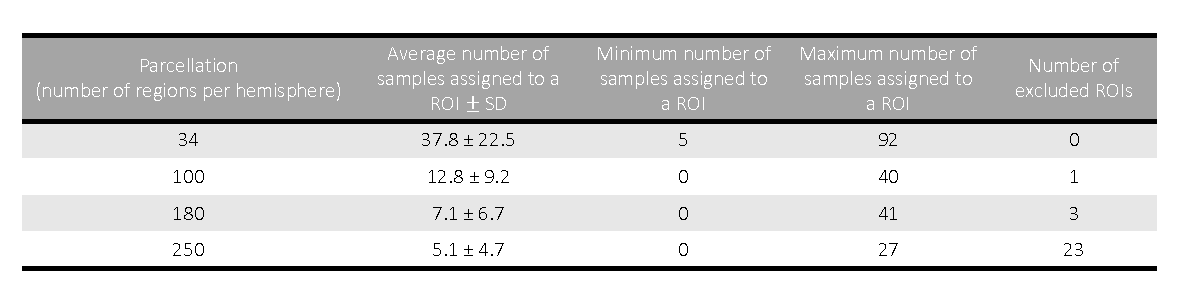
\includegraphics[width=1\textwidth]{Chapter4/TableS4.pdf}
\label{TableS4}
\end{figure}

\section{Evaluating distances between samples}
\label{app:AppendixCh4_5}

All distances between samples were calculated on a set of samples that were mapped onto individual parcellations applying a $2\,$mm distance threshold as described in Step 4. Voxel coordinates provided by the AHBA that were used to map samples to subject-specific parcellations are derived from images in subject space and could not be combined to estimate distances between samples from different subjects. Therefore, for both Euclidean distances and distances within cortical surfaces we used MNI coordinates provided by the AHBA for each region to estimate the pairwise distances between them given that MNI coordinates are derived in the same space for all subjects.

\textbf{Euclidean distances} were calculated using the function \texttt{pdist2} in MATLAB 2016b\footnote{MATLAB is a product of Mathworks}.

\textbf{Distances within cortical volume} were calculated using an HCPMMP1 \citep{Glasser2016} parcellation in the MNI space (downloaded from \url{https://neurovault.org/collections/1549/}, file \texttt{MMP\_in\_MNI\_corr.nii})  by: i) changing the strides of the image from $[-1 3 -2]$ to $[-1 2 3]$ in order to change the image orientation; ii) rendering the brain parcellation in MNI space as a 3D matrix; iii) converting the original MNI sample coordinates to voxel-based coordinates that correspond to the parcellation loaded in a 3D matrix format; iv) finding the closest coordinate in the parcellation for each sample and mapping a sample to that location; v) rendering the parcellation as a graph with each voxel representing a node; vi) implementing Dijkstra’s algorithm \citep{Dijkstra1959} to calculate the closest distances between samples within the GM volume using \texttt{shortestpath} function in MATLAB. Distances between pairs of regions were calculated as an average of distances between samples within them.

\textbf{Distance on the cortical surface} were calculated using annotation files for each parcellation and the spherical representation of the cortical surface by: i) identifying vertices that correspond to a particular region on the sphere and calculating the mean of their coordinates to obtain a centroid value; ii) mapping centroid coordinates to the cortical surface representation; iii) calculating the distances between each pair of regions using the \texttt{toolbox\_fast\_marching} toolbox in MATLAB.


\section{Spatial relationship between CGE and distance}
\label{app:AppendixCh4_6}

Figure \ref{fig:Ch4Sfig9}B shows the relationship between CGE and separation distance for three different types of regional pairs: (i) intra-cortical region pairs, which show relatively high CGE at all distances (light grey); (ii) intra-subcortical region pairs, which show a linearly decreasing relationship at short distances (dark grey); and (iii) cortical-subcortical region pairs, which demonstrate mostly negative CGE at all distances (peach). This variability precludes simple removal of a global trend as in \citep{Fulcher2016} and suggests a separate correction should be applied for each class of connection. Figure \ref{fig:Ch4Sfig9}C shows the result of removing the mean CGE at each equiprobable distance bin separately for each connection class. Even after this correction, intracortical CGE values appear to be underestimated while cortico-subcortical are overestimated. Another method for addressing the inherent differences between cortical and subcortical gene expression profiles is to normalize the expression data separately for these two anatomical divisions [e.g., \citet{Anderson2018}]. With this approach, expression values are scaled relative to other values within just the cortex, or within just the subcortex. Division-specific normalization allows a gene to score highly if its expression in the subcortex is high relative to other subcortical regions, even if its expression relative to the cortex may be low (and vice-versa), at the expense of distorting the magnitude relationships between cortical and subcortical values. With this approach, the negative correlation between cortical and subcortical regions is reduced with some region pairs demonstrating relatively similar gene expression profiles (Figure \ref{fig:Ch4Sfig9}D). As presented in Figure \ref{fig:Ch4Sfig9}E, the relationship between CGE and separation distance is now more qualitatively similar for all three groups and can be corrected using simple mean subtraction across distance bins (Figure \ref{fig:Ch4Sfig9}F).


\section{API: probe sequences}
\label{app:AppendixCh4_7}

\textbf{API: probe sequences} for the first \num{10000} rows.\\
\url{http://api.brain-map.org/api/v2/data/query.xml?criteria=model::Probe,rma::criteria,products[id$eq2],rma::include,gene,predicted_sequence,rma::options[only$eq%27probes.name,probes.type,probes.ncbi_accession_number,probes.gi,genes.entrez_id,genes.acronym,sequences.sequence_length,sequences.sequence_data%27],[num_rows$eq10000][start_row$eq0]}

\newpage
\section{Supplementary figures}

\begin{figure}[h!]
  \centering
    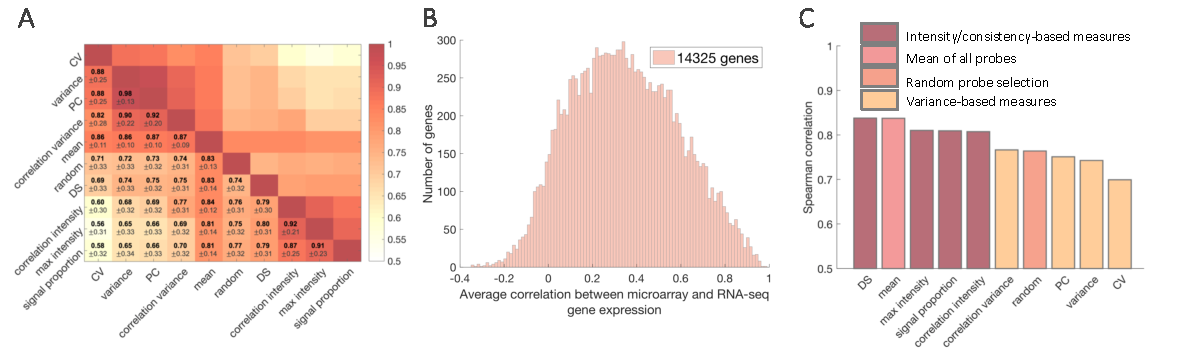
\includegraphics[width=1\textwidth]{Chapter4/FigureS1.pdf}
\caption{\textbf{Average correlation between summary expression scores for genes annotated to multiple probes, where a single representative probe is chosen based on different criteria after intensity-based filtering (IBF).}
(A) Average correlation between summary expression scores for genes annotated to multiple probes, where a single representative probe is chosen based on different criteria: CV, variance, PC, signal proportion, DS, correlation variance, correlation intensity, mean (see Table \ref{Table2}) or selecting a representative probe at random (correlation values averaged over $100$ runs). The average correlation is computed over \num{11190} genes with multiple probe annotations after intensity-based filtering. 
(B) The distribution of Spearman correlation coefficients between microarray and RNA-seq expression data for genes that are present in both datasets. When multiple probes for a gene were available, the maximum correlation value between probes was selected. IBF increases the average correlation between microarray and RNA-seq gene expression measures relative to not using IBF, Wilcoxon rank-sum test, $p=1.1 \times 10^{-49}$. 
(C) Average correlation between probes selected using RNA-seq expression (by selecting the probe that is correlated to the RNA-seq data the most) and other methods (ordered by decreasing values, based on \num{7950} genes that (i) were present in both microarray and RNA-seq datasets; (ii) were correlated to RNA-seq in excess of a threshold value ($\rho > 0.2$, Spearman rank correlation) to ensure that RNA-seq based probe selection provides a meaningful estimate of the microarray measures; (iii) had more than one probe available after intensity-based filtering). }
\label{fig:Ch4Sfig1}
\end{figure}

\begin{figure}[h!]
  \centering
    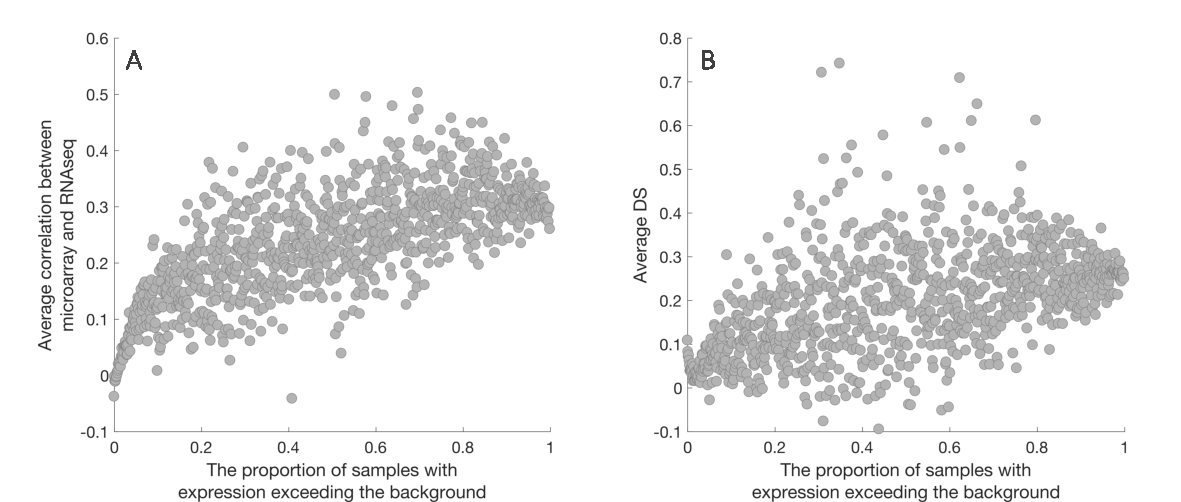
\includegraphics[width=1\textwidth]{Chapter4/FigureS2.pdf}
\caption{\textbf{The effect of intensity based filtering.}
The relationship between the proportion of samples with expression measures exceeding the background and 
(A) the average correlation between microarray and RNA-seq expression measures at the probe level (Spearman's $\rho = 0.3$, $p<0.001$); 
(B) the average differential stability (DS) for each gene (Spearman's $\rho = 0.33$, $p<0.001$). DS measures were calculated based on the scaled robust sigmoid normalized data (see Eq.\ref{eqn:eq2}) within the regions of the left cortex. Correlation and differential stability values are averaged within 1000 bins to aid visualization.}
\label{fig:Ch4Sfig2}
\end{figure}

\begin{figure}[h!]
  \centering
    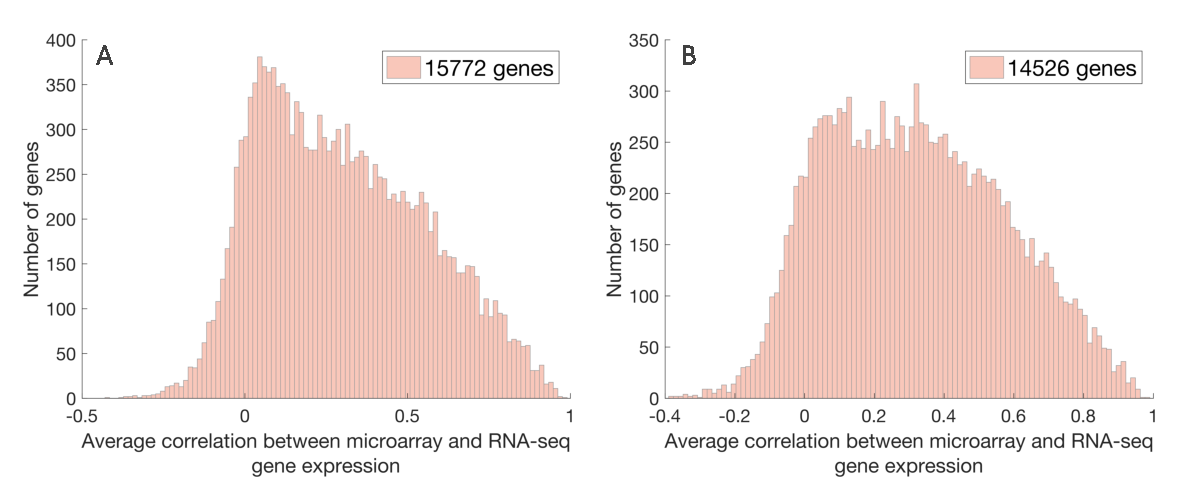
\includegraphics[width=1\textwidth]{Chapter4/FigureS3.pdf}
\caption{\textbf{Correlation to RNA-seq expression measures and gene expression measures obtained following variance-based filtering of probes.}
In variance-based filtering probes with the lowest variance are to be excluded. A probe was excluded if it was consistently classified within the $50\%$ of the  lowest variance probes in all six brains. This figure shows the distribution of Spearman correlation values between microarray and RNA-seq expression data for genes that are present in both datasets when the variance-based filtering is applied to $\log_2$-transformed data (A) and non-transformed data (B). We use RNA-seq data as a gold standard to verify microarray filtering results. When multiple probes for a gene were available, the probe with the maximum correlation value was selected. Variance-based filtering on $\log_2$-transformed data decreases the correlation between microarray and RNA-seq expression measures compared to the data prior to filtering (Wilcoxon rank-sum test, $p = 10^{-5}$). Variance-based filtering on non-transformed data increases the mean correlation (Wilcoxon rank-sum test, $p = 0.008$), but the increase is not as large as when using intensity-based filtering (see Figure \ref{fig:Ch4Sfig1}).}
\label{fig:Ch4Sfig3}
\end{figure}

\begin{figure}[h!]
  \centering
    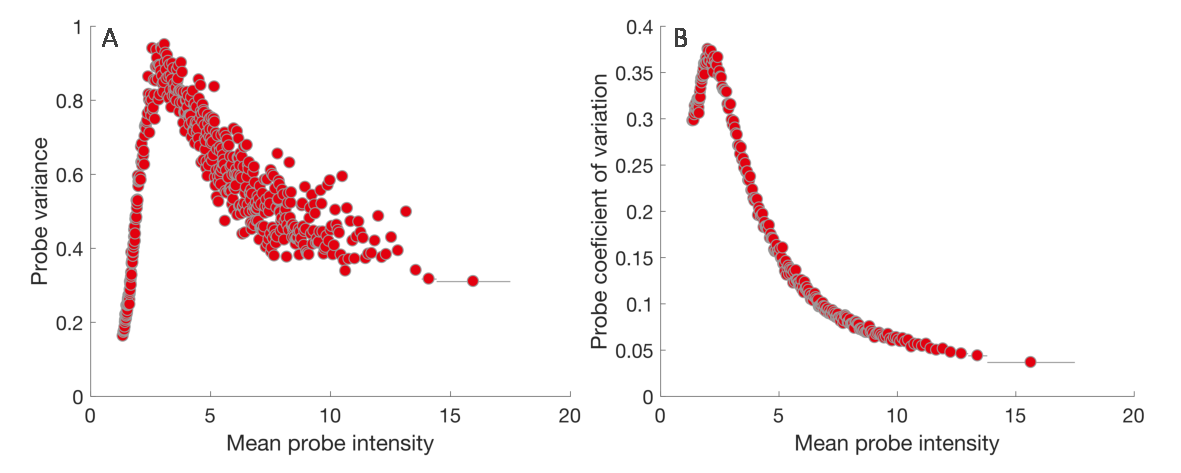
\includegraphics[width=1\textwidth]{Chapter4/FigureS4.pdf}
\caption{\textbf{The relationship between average probe intensity, variance, and coefficient of variation.}
The relationship between average probe intensity and (A) variance, and (B) coefficient of variation in 500 and 250 equiprobable intensity bins respectively, shown as a circle (bin centers) and a horizontal line (bin extent). The relationship between probe intensity and variance is positive for low intensity probes (intensity$<3$); for higher intensity probes increasing intensity results in decreasing variance. The same trend is evident for the relationship between coefficient of variation and intensity.}
\label{fig:Ch4Sfig4}
\end{figure}

\begin{figure}[h!]
  \centering
    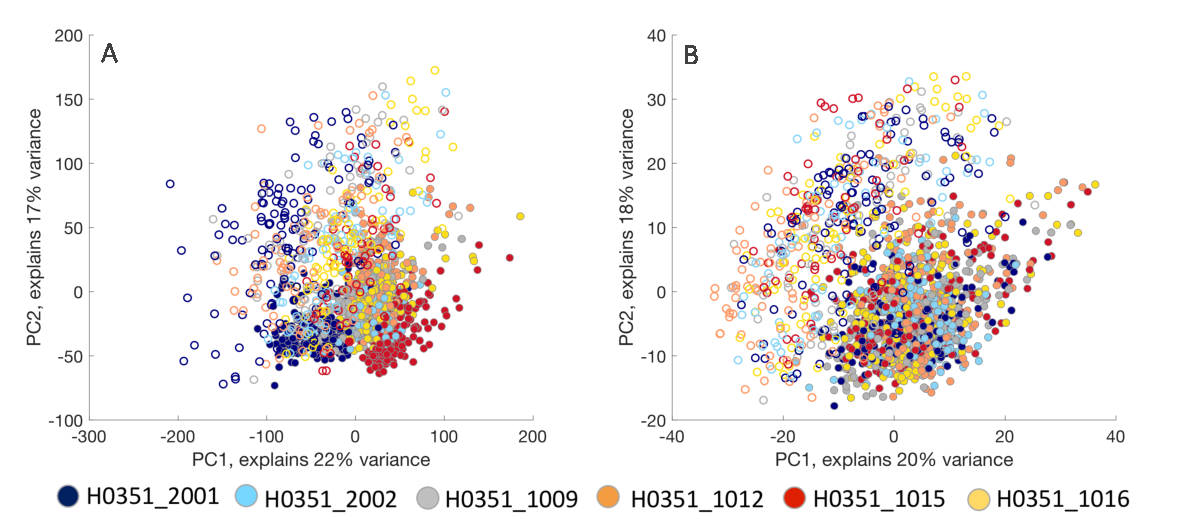
\includegraphics[width=1\textwidth]{Chapter4/FigureS5.pdf}
\caption{\textbf{Inter-individual differences in gene expression and the effect of normalization in the whole brain.}
(A) Original gene expression data for cortical and subcortical samples in principal component space. Data from different donors are represented in different colours. Samples from different subjects occupy different parts of the low-dimensional gene expression space. 
(B) gene expression data in principal component space normalized using scaled robust sigmoid (SRS). After normalization samples no longer segregate by donor and show a more clear separation between cortex and subcortex. Filled and closed markers denote cortical and subcortical regions, respectively.}
\label{fig:Ch4Sfig5}
\end{figure}

\begin{figure}[h!]
  \centering
    \includegraphics[width=1\textwidth]{Chapter4/FigureS6.pdf}
\caption{\textbf{A schematic representation of cross-gene and cross-sample normalization.} Within-sample cross-gene normalization estimates the relative expression level of all available genes within a given sample (grey row). Within-gene cross sample normalization estimates the relative expression of a particular gene across all available samples (red column).}
\label{fig:Ch4Sfig6}
\end{figure}

\begin{figure}[h!]
  \centering
    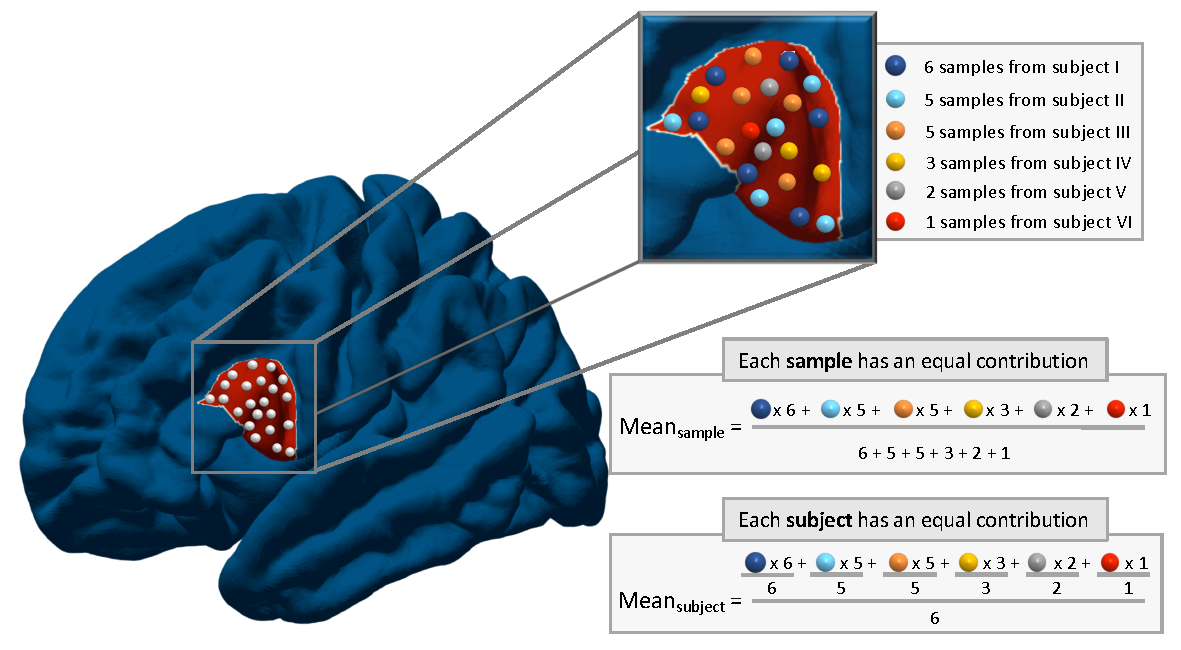
\includegraphics[width=1\textwidth]{Chapter4/FigureS7.pdf}
\caption{\textbf{Two alternative ways of averaging expression values within the region of interest.}
Each region of interest might contain a different number of samples from each subject. For example, the presented region has 6 samples from subject I, 5 samples from subjects II and III, 3 samples from subject IV and only 2 and 1 samples from subjects V and VI respectively. One way of calculating the mean is to take the average of all samples, such that each sample makes an equal contribution to the overall expression value ($\mathrm{Mean_{sample}}$). An alternative is to average the samples from each donor first, and then take a second-order average across donors ($\mathrm{Mean_{subject}}$). The latter ensures that each subject makes an equal contribution to the summary expression value. The former might be influenced by donors with more samples in a given region. The choice of inter-subject averaging does not significantly impact the statistics in the reported study. As an example, for the cortical parcellation containing 180 regions per hemisphere, we compare data using both sample and subject-level averaging. The mean correlation between resulting regional expression vectors (for each region across all genes) is $0.97$ ($SD = 0.04$). The lowest correlation (outlier) is $0.76$ for one region, which contains samples from three subjects [S1($n=2$), S2($n=6$), S5($n=1$)]. In this region, S2 dominates the mean if the average across samples is taken. The mean correlation between gene expression measures (for each gene across regions) is also $0.97$ ($SD = 0.01$) with no obvious outliers. These findings suggest that different averaging approaches are likely to have a minor effect on study findings at a global level, but could affect regionally-focused analyses; particularly regions with an uneven distribution of samples across donors.}
\label{fig:Ch4Sfig7}
\end{figure}

\begin{figure}[h!]
  \centering
    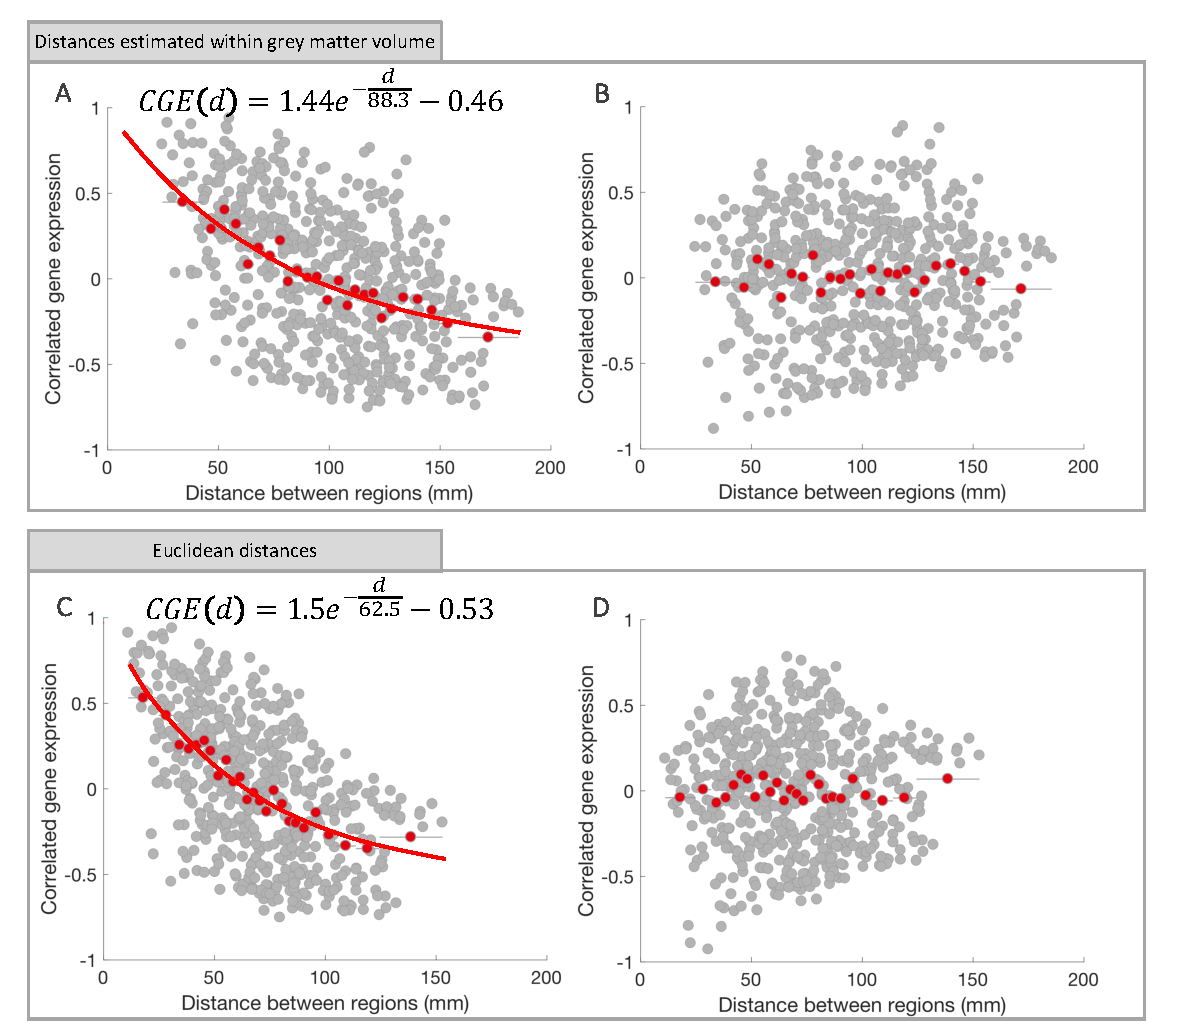
\includegraphics[width=1\textwidth]{Chapter4/FigureS8.pdf}
\caption{\textbf{The relationship between CGE and inter-regional distance estimated within grey matter volume and as Euclidean distance.}
Top: the relationship between CGE and distance when the distance between regions calculated within grey matter volume. Bottom: the relationship between CGE and distance when the distance between regions calculated as Euclidean distance. A,C) CGE as a function of separation distance where CGE between pairs of regions are represented in grey dots and red dots represent the mean value in 25 equiprobable distance bins; The red line represents an exponential fit. A) $CGE(d) = 1.44e^{-d/88.3}-0.46$; C) $CGE(d)=1.5e^{-d/62.5}-0.53$.
B,D) Residuals after removing the exponential trend in each case;
CGE calculated using all \num{10027} genes (after intensity-based filtering and probe selection based on correlation to RNA-seq data). }
\label{fig:Ch4Sfig8}
\end{figure}

\begin{figure}[h!]
  \centering
    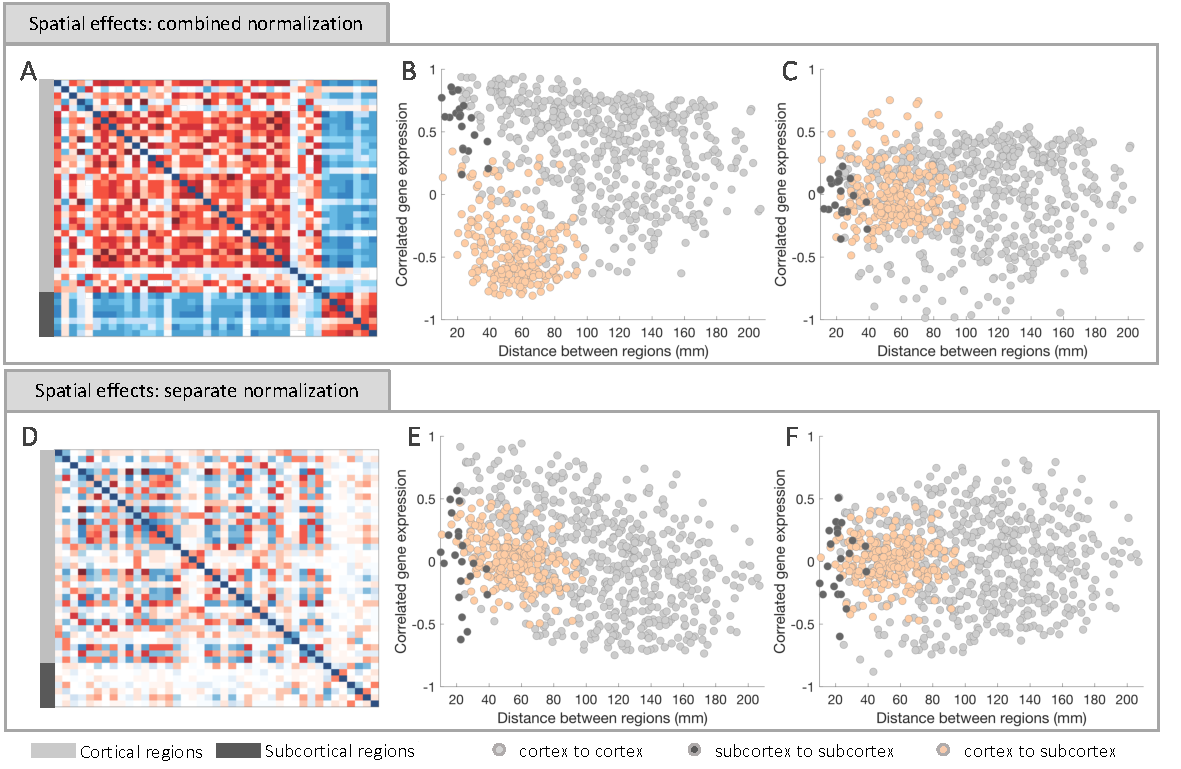
\includegraphics[width=1\textwidth]{Chapter4/FigureS9.pdf}
\caption{\textbf{The relationship between CGE and inter-regional distance for cortical and subcortical regions.}
Top row: 
(A) Matrix of CGE values for the left hemisphere, including both cortical and subcortical regions, in which expression values have been normalized for both cortical and subcortical regions together; 
(B) CGE as a function of separation distance where CGE between different subsets of regions are represented in different colours: within cortex -- light grey, within subcortex -- dark grey, between cortex and subcortex -- peach; 
(C) CGE residuals after removing the spatial effect for each subset of regions separately by subtracting the average of each bin, where different colours represent subsets of connections as above. 
(D) Matrix of CGE values for the left hemisphere, including both cortical and subcortical regions, in which expression values have been normalized separately for cortical and subcortical regions; 
(E) CGE as a function of separation distance, where normalization has been performed on cortical and subcortical regions separately. Different colours represent subsets of connections as above; 
(F) CGE residuals after removing the spatial effect for each subset of regions (when normalization performed on cortical and subcortical regions separately) by subtracting the average of each bin where different colours represent subsets of connections as above. Distances between cortical regions were evaluated on the cortical surface while distances between subcortical regions as well as between cortical and subcortical regions estimated as Euclidean.}
\label{fig:Ch4Sfig9}
\end{figure}

\begin{figure}[h!]
  \centering
    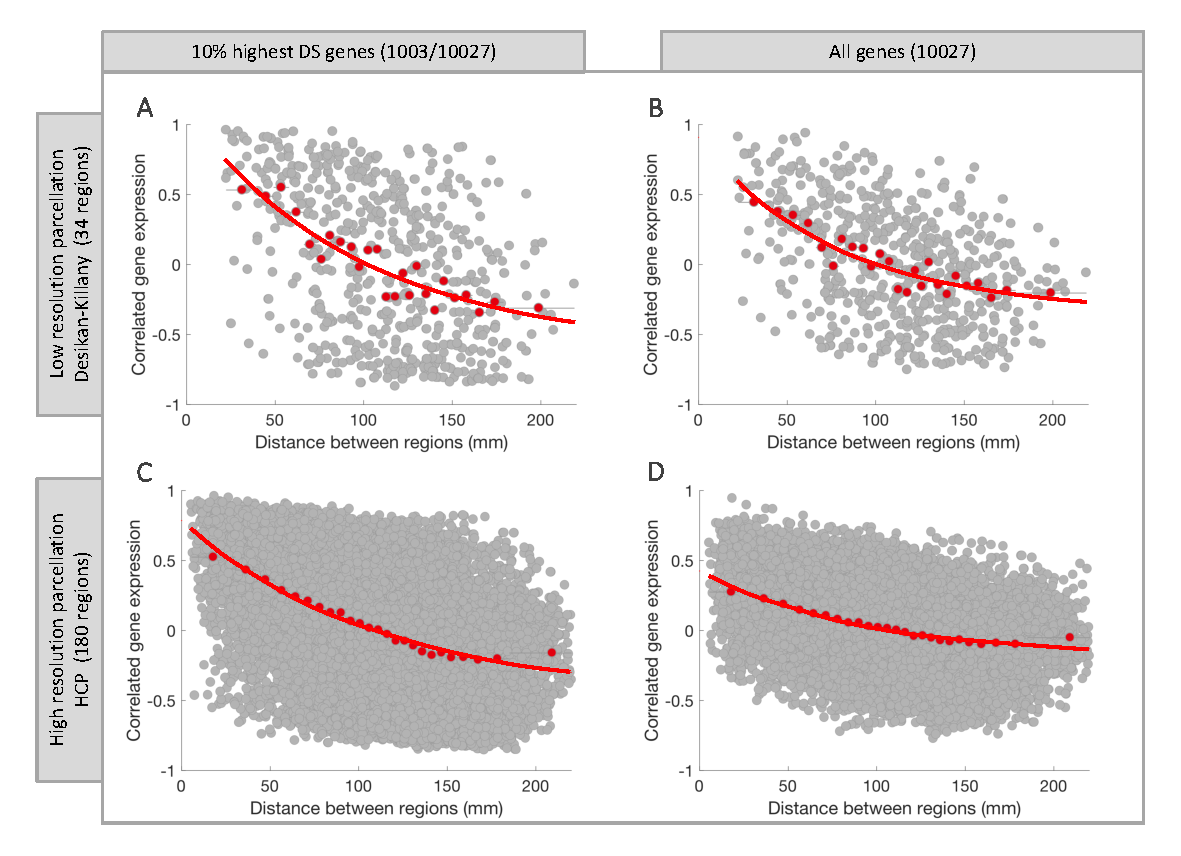
\includegraphics[width=1\textwidth]{Chapter4/FigureS10.pdf}
\caption{\textbf{The relationship between CGE and inter-regional distance on the cortical surface for high and low resolution parcellations using a full set of genes and a set of only highest DS genes.}
The relationship between CGE and inter-regional distance for different resolution cortical parcellations and different sets of genes. Top row: low resolution Desikan-Killany parcellation \citep{Desikan2006} ($34$ regions). Bottom row: high resolution HCPMMP1 \citep{Glasser2016} parcellation ($180$ regions). First column: CGE calculated using only $10\%$ of highest DS genes that are most consistently expressed across subjects and regions. Second column: CGE calculated using all \num{10027} genes. The relationship between CGE and inter-regional distance also depends on the subset of genes chosen for the calculation, such that high DS genes show a stronger association with inter-regional distance. This effect is more pronounced in the higher resolution parcellation.}
\label{fig:Ch4Sfig10}
\end{figure}
